% Verification Gap Ledger preprint.
% Every number is a macro from numbers.tex and every data table is an input file; both are
% written by code/06_preprint_assets.py from the released data. Build: latexmk -pdf vgl_preprint.tex
\documentclass[10pt,twocolumn,letterpaper]{article}
\usepackage[T1]{fontenc}
\usepackage[utf8]{inputenc}
\usepackage{mathpazo}
\usepackage{amsmath,amssymb}
\usepackage[letterpaper,top=0.85in,bottom=0.9in,left=0.72in,right=0.72in,columnsep=0.28in]{geometry}
\usepackage{graphicx}
\usepackage{booktabs}
\usepackage{tabularx}
\usepackage{array}
\usepackage{xcolor}
\usepackage[numbers,sort&compress]{natbib}
\usepackage[labelsep=colon,font=small,justification=centering,skip=4pt]{caption}
\usepackage{titlesec}
\usepackage{enumitem}
\usepackage{microtype}
\usepackage{xurl}
\urlstyle{same}
\usepackage[colorlinks=true,linkcolor={red!65!black},citecolor={blue!60!black},urlcolor={blue!60!black}]{hyperref}

% Generated by code/06_preprint_assets.py from stats.json and stats_preprint.json. Do not edit.
\newcommand{\nProg}{24}
\newcommand{\nFed}{15}
\newcommand{\nNY}{9}
\newcommand{\nEvid}{80}
\newcommand{\nRzero}{2}
\newcommand{\nRone}{9}
\newcommand{\nRtwo}{8}
\newcommand{\nRthree}{3}
\newcommand{\nRfour}{2}
\newcommand{\nCzero}{12}
\newcommand{\nCone}{5}
\newcommand{\nCtwo}{5}
\newcommand{\nCthree}{1}
\newcommand{\nCfour}{1}
\newcommand{\nAzero}{16}
\newcommand{\nAone}{6}
\newcommand{\nAtwo}{2}
\newcommand{\nAthree}{0}
\newcommand{\nRleOne}{11}
\newcommand{\pctRleOne}{46}
\newcommand{\nRgeThree}{5}
\newcommand{\pctRgeThree}{21}
\newcommand{\pctCzero}{50}
\newcommand{\pctAzero}{67}
\newcommand{\nAleOne}{22}
\newcommand{\pctAleOne}{92}
\newcommand{\nBoth}{0}
\newcommand{\nGapPos}{14}
\newcommand{\pctGapPos}{58}
\newcommand{\nGapNeg}{5}
\newcommand{\nGapZero}{5}
\newcommand{\meanR}{1.75}
\newcommand{\meanC}{0.92}
\newcommand{\meanA}{0.42}
\newcommand{\meanOG}{2.00}
\newcommand{\tauRC}{0.19}
\newcommand{\pRC}{0.30}
\newcommand{\tauRA}{0.70}
\newcommand{\tauCA}{0.26}
\newcommand{\pCA}{0.16}
\newcommand{\rtemElec}{20}
\newcommand{\rtemFossil}{42}
\newcommand{\rtemComb}{24}
\newcommand{\nLowR}{9}
\newcommand{\nLowC}{5}
\newcommand{\nLowA}{8}
\newcommand{\nLowRState}{6}
\newcommand{\nTermContested}{2}
\newcommand{\nModified}{2}
\newcommand{\scBothAfter}{5}
\newcommand{\scGapAfter}{11}
\newcommand{\scCzeroAfter}{11}
\newcommand{\scMeanCAfter}{1.33}
\newcommand{\scAffected}{5}
\newcommand{\sensRleOneMin}{6}
\newcommand{\sensRleOneMax}{15}
\newcommand{\sensAleOneMin}{21}
\newcommand{\sensBProg}{10}
\newcommand{\sensBAleOne}{9}
\newcommand{\accessDate}{2026-10-11}
\newcommand{\vglVersion}{0.1.0}

\makeatletter\newcommand{\tabinput}[1]{\@@input #1 }\makeatother

% ---- physics-preprint conventions: TABLE I above, FIG. 1 below, Roman section numbers
\renewcommand{\thetable}{\Roman{table}}
\captionsetup[table]{name=TABLE,position=top}
\captionsetup[figure]{name=FIG.}
\renewcommand{\thesection}{\Roman{section}}
\renewcommand{\thesubsection}{\Alph{subsection}}
\titleformat{\section}{\normalfont\small\bfseries\filcenter}{\thesection.}{0.6em}{\MakeUppercase}
\titlespacing*{\section}{0pt}{1.6ex plus .5ex}{1.0ex}
\titleformat{\subsection}{\normalfont\small\bfseries\filcenter}{\thesubsection.}{0.5em}{}
\titlespacing*{\subsection}{0pt}{1.3ex plus .4ex}{0.8ex}
\setlength{\parindent}{1.2em}
\setlength{\bibsep}{1.5pt}
\renewcommand{\bibfont}{\footnotesize}
\setlist{nosep,leftmargin=1.4em}
\newcolumntype{L}[1]{>{\raggedright\arraybackslash}p{#1}}
\newcommand{\R}{R}\newcommand{\C}{C}\newcommand{\A}{A}

\begin{document}

\twocolumn[{
\begin{center}
{\large\bfseries Measuring the verification gap in municipal energy and infrastructure funding:\\[2pt] a source-coded register of federal and New York State programs}\\[10pt]
{\normalsize Stephen Olumide Akindipe\,\href{https://orcid.org/0000-0002-1846-9662}{\raisebox{0.5pt}{\scriptsize\textcolor{green!45!black}{\textsuperscript{iD}}}}}\\[2pt]
{\small\itshape Independent Researcher, Albany, New York, USA}\\[1pt]
{\small ORCID \href{https://orcid.org/0000-0002-1846-9662}{0000-0002-1846-9662}}\\[1pt]
{\small Data: Verification Gap Ledger v\vglVersion, \href{https://doi.org/10.5281/zenodo.23302898}{doi:10.5281/zenodo.23302898}}\\[8pt]
\begin{minipage}{0.86\textwidth}
\small
Federal and New York State programs that fund municipal energy and infrastructure projects routinely state expected energy, cost, emissions, and resilience benefits. Whether those benefits can later be confirmed depends on three design features that are rarely recorded together: what proof of results a program requires of recipients, what results the program makes public, and whether the resulting data could support attribution of outcomes to the funding. We introduce the Verification Gap Ledger, an open and versioned register that codes programs on three ordinal scales, required verification ($R$, 0 to 4), public results ($C$, 0 to 4), and outcome attributability ($A$, 0 to 3), with every code tied to a cited source document and locator. Version \vglVersion{} covers \nProg{} programs (\nFed{} federal, \nNY{} New York State) supported by \nEvid{} evidence items. In this sample, \nRleOne{} programs (\pctRleOne{} percent) require no more than output reporting and \nRgeThree{} (\pctRgeThree{} percent) require measured or independently verified outcomes; none of those \nRgeThree{} publishes project-level outcome data. In addition, \nCzero{} programs (\pctCzero{} percent) publish no results beyond award announcements, \nAleOne{} (\pctAleOne{} percent) are coded at or below a modeled baseline for attributability, and none uses a comparison group or formal impact design. The two programs that publish project-level outcomes report modeled estimates. Required verification and public results are weakly associated (Kendall's $\tau_b = \tauRC$, $p = \pRC$), while required verification and attributability are strongly associated ($\tau_b = \tauRA$, $p < 0.001$). Where independent measurement exists it diverges from estimates: a billing-analysis evaluation of one New York program found a gross electric realization rate of \rtemElec{} percent. The central finding, that no program both measures and publishes project-level outcomes, holds under every treatment of low-confidence codes that we test. An illustrative scenario in which programs that already measure outcomes publish them shows how the register can be used to evaluate disclosure policy.\\[4pt]
\textbf{Keywords:} measurement and verification, program evaluation, municipal energy, infrastructure finance, performance reporting, transparency, open data
\end{minipage}
\end{center}
\vspace{10pt}
}]

% =====================================================================
\section{Introduction}

Public funding for municipal energy and infrastructure in the United States has expanded substantially since 2021. The Infrastructure Investment and Jobs Act (IIJA) \cite{iija2021} and the Inflation Reduction Act (IRA) \cite{ira2022} created or recapitalized programs for building efficiency, grid resilience, electric vehicle charging, clean school buses, water infrastructure, and hazard mitigation, and opened direct payment of clean energy tax credits to state and local governments. New York State operates a parallel portfolio through the New York State Energy Research and Development Authority (NYSERDA), the Department of Environmental Conservation (NYSDEC), the Environmental Facilities Corporation (EFC), and the New York Power Authority (NYPA). Municipalities are eligible recipients, subrecipients, borrowers, or participants in many of these programs.

These programs are justified in part by expected outcomes: kilowatt hours saved, emissions avoided, outage minutes reduced, losses avoided. The credibility of those expected outcomes depends on what happens after the award. A program can require recipients to report only financial information, to count delivered outputs, to estimate outcomes with deemed or modeled values, to measure outcomes against a baseline, or to submit measurement to an independent party. Separately, a program may publish nothing, publish totals, or publish project-level data that others can analyze. Finally, the data a program collects may or may not support a defensible claim that the funding caused the observed result.

These three properties are distinct, and they need not move together. A program can collect metered data and publish none of it; another can publish detailed project records that contain only modeled estimates. Yet municipal officials choosing among funding sources, auditors reviewing performance claims, and researchers studying program effects have no single public record of how programs differ on these dimensions. Each program's requirements are spread across statutes, regulations, notices of funding opportunity, reporting templates, compliance supplements, program pages, and evaluation reports.

Measurement and verification (M\&V) is the established practice for determining the savings of an energy project. The International Performance Measurement and Verification Protocol (IPMVP) defines savings as the difference between measured post-project consumption and an adjusted baseline, with options ranging from partial measurement of retrofitted equipment to whole-facility utility bill analysis \cite{evo2022}. M\&V performed by a party independent of the recipient is the strongest form of verification short of an impact evaluation. Much program reporting relies instead on deemed savings, engineering calculations, or applicant projections. These are useful for planning, but they are estimates, not measurements.

A body of empirical work compares projected and realized savings in publicly supported programs. Allcott and Greenstone argued that the engineering estimates commonly used to justify efficiency programs are an unreliable guide to realized savings and called for more rigorous ex post evaluation \cite{allcott2012}. Using a randomized encouragement design in the federal Weatherization Assistance Program, Fowlie, Greenstone, and Wolfram found that projected savings substantially exceeded realized savings \cite{fowlie2018}. Davis, Fuchs, and Gertler found smaller than expected savings in a large appliance replacement program \cite{davis2014}, and Christensen and coauthors decomposed the gap between projected and realized returns into components attributable to engineering models, installation quality, and behavior \cite{christensen2023}. A common finding is that the size of the gap is unknown until measurement is performed, and that measurement is often absent from routine program reporting.

Showing that a measured change was caused by funding requires a counterfactual. Measured pre and post comparisons at project level control for some but not all confounders, such as weather, occupancy, and concurrent changes. Comparison group, randomized, or quasi-experimental designs, and net-to-gross adjustments in utility program evaluation, address attribution more directly \cite{gertler2016}. The data a program requires therefore determine whether such analysis is possible after the fact: a program that collects no baseline cannot support attribution, regardless of later analytical effort.

Federal performance management law requires agencies to set goals and report on them \cite{gpra2010} and to build evidence about program effectiveness \cite{evidenceact2018}. For individual awards, the Uniform Guidance requires periodic performance reports relating accomplishments to award objectives, at least annually, but it recommends rather than requires that awards specify baselines and outcome indicators \cite{cfr200}. Research on performance management has long noted the distance between outputs that are easy to count and outcomes that matter \cite{heinrich2002,moynihan2008}. Research on transparency policy shows that disclosure is effective only when the information disclosed is usable by its intended audience \cite{fung2007,hood2006}; open, machine-readable release is one condition for usability, consistent with the FAIR principles for research data \cite{wilkinson2016}.

This literature evaluates individual programs or describes general reporting obligations. It does not provide a cross-program register that records, for each program and with source citations, what verification is required, what is published, and whether attribution is possible. We contribute that register, the Verification Gap Ledger (VGL) \cite{akindipe2026vgl}. The approach follows a familiar pattern in applied evaluation, in which a program's stated objectives are compared with what its design can deliver or demonstrate using transparent, reproducible indicators \cite{delmelle2012}; here the indicators concern evidence rather than access. The Ledger does not estimate program effects. It records the evidentiary conditions under which program effects could be estimated by others.

The paper is organized as follows. In Sec.~\ref{sec:framework} we set out the coding framework formally, including the three scales, the derived measures, the association statistic, and the operators used for sensitivity analysis and scenario evaluation. Section~\ref{sec:data} describes the study scope, the program sample, the source hierarchy, the decision rules, and the reproducible pipeline. Section~\ref{sec:results} reports results. Section~\ref{sec:interp} interprets them through a sensitivity analysis, an illustrative disclosure scenario, and policy implications. Section~\ref{sec:limits} states limitations, and Sec.~\ref{sec:concl} concludes and sets out the release schedule.

% =====================================================================
\section{The verification gap framework}\label{sec:framework}

This section defines the quantities used throughout the paper. Let $\mathcal{P}$ denote the set of coded programs, with $n = |\mathcal{P}| = \nProg$ in version \vglVersion. Each program $i \in \mathcal{P}$ receives one code on each of three ordinal scales,
\begin{equation}
R_i \in \{0,\dots,4\}, \qquad C_i \in \{0,\dots,4\}, \qquad A_i \in \{0,\dots,3\},
\label{eq:scales}
\end{equation}
where $R_i$ records the verification of results that the program's rules require of recipients, $C_i$ records the results that any member of the public can see, and $A_i$ records whether the required or published data could support attribution of outcomes to the funding. The levels of each scale and the test that assigns them are given in Table~\ref{tab:scales}.

\begin{table*}[t]
\caption{Coding scales of the Verification Gap Ledger. Source: docs/CODEBOOK.md, Verification Gap Ledger v\vglVersion.}
\label{tab:scales}
\footnotesize
\begin{tabularx}{\textwidth}{L{2.6cm} c L{3.6cm} X}
\toprule
Scale & Code & Label & Test \\
\midrule
$R$, required verification & 0 & Financial only & Only financial reports or eligibility documentation required \\
 & 1 & Outputs & Recipients report activities or units delivered \\
 & 2 & Estimated outcomes & Outcome quantities are modeled, deemed, projected, or calculated \\
 & 3 & Measured outcomes against a baseline & Outcomes from meters, bills, or operating records, against a baseline or measured operating performance \\
 & 4 & Independent verification & M\&V or impact evaluation by a party independent of the recipient \\
\midrule
$C$, public results & 0 & No public results & No public release of results; award announcements and recipient lists do not count \\
 & 1 & Aggregate only & Program totals or evaluation summaries only \\
 & 2 & Project-level outputs & Outputs published per project or recipient \\
 & 3 & Project-level outcomes & Outcome quantities (estimated or measured) published per project \\
 & 4 & Machine-readable open project data & Project-level outcome fields as bulk machine-readable data with open terms \\
\midrule
$A$, outcome attributability & 0 & No baseline & No baseline required or published \\
 & 1 & Baseline or modeled counterfactual only & A baseline exists but results are not measured against it, or the counterfactual is modeled \\
 & 2 & Measured pre and post & Measured outcomes before and after, at project level \\
 & 3 & Comparison group or impact evaluation & Comparison group, randomized or quasi-experimental design, or net-to-gross impact evaluation \\
\bottomrule
\end{tabularx}
\end{table*}

\subsection{Derived measures}

Two derived measures summarize each program. The required-to-public gap is
\begin{equation}
G_i = R_i - C_i ,
\label{eq:gap}
\end{equation}
which is positive when the rules ask for more proof than is published and negative when more is published than the rules require. The outcome gap is
\begin{equation}
O_i = 4 - \max(R_i, C_i),
\label{eq:og}
\end{equation}
which measures distance from the highest evidence level reached on either the requirement or the disclosure scale, with $O_i = 0$ best. Both measures subtract ordinal codes for convenience. A difference of 2 is not interpreted as twice a difference of 1, and means of codes are reported only as summaries.

Headline indicators are counts and shares of programs satisfying a condition $\phi$,
\begin{equation}
N(\phi) = \sum_{i \in \mathcal{P}} \mathbf{1}[\phi(i)], \qquad s(\phi) = \frac{N(\phi)}{n},
\label{eq:share}
\end{equation}
for the five conditions $R_i \le 1$ (outputs or less), $R_i \ge 3$ (measured or independently verified), $C_i = 0$ (no public results), $A_i \le 1$ (at or below a modeled baseline), and the joint condition $R_i \ge 3 \wedge C_i \ge 3$, which identifies programs that both measure and publish project-level outcomes. The count $N(G_i > 0)$ of programs with a positive gap and the mean outcome gap $\bar{O} = n^{-1}\sum_i O_i$ complete the set.

\subsection{Evidence and confidence}

Let $\mathcal{E}_i^d$ be the set of evidence items recorded for program $i$ on dimension $d \in \{R, C, A\}$, and let each item $e$ carry a code $c(e)$ and a confidence $q(e) \in \{\text{low} < \text{medium} < \text{high}\}$: high when the rule text was read directly, medium for an official secondary description or partial text, and low when the code is inferred from incomplete official material. Every assigned code must be supported by at least one item, and the confidence of a program on a dimension is the strongest support for the code assigned,
\begin{equation}
\kappa_i^d = \max \left\{ q(e) : e \in \mathcal{E}_i^d,\; c(e) = d_i \right\}.
\label{eq:conf}
\end{equation}
The release pipeline rejects any program for which this set is empty.

\subsection{Association between scales}

Because the codes are ordinal with many ties, associations are summarized with Kendall's $\tau_b$ \cite{kendall1945}. For two scales $X$ and $Y$ observed on the same $n$ programs,
\begin{equation}
\tau_b = \frac{n_c - n_d}{\sqrt{(n_0 - n_X)(n_0 - n_Y)}},
\label{eq:tau}
\end{equation}
where $n_c$ and $n_d$ are the numbers of concordant and discordant pairs, $n_0 = n(n-1)/2$, and $n_X = \sum_k t_k(t_k-1)/2$ and $n_Y = \sum_l u_l(u_l-1)/2$ count pairs tied on $X$ and on $Y$, with $t_k$ and $u_l$ the sizes of the tied groups. Two-sided $p$-values use the asymptotic normal approximation as implemented in SciPy \cite{virtanen2020}. Given the small and purposive sample, the coefficients are descriptive.

\subsection{Realization rate}

For a program with an independent evaluation, the gross realization rate is the ratio of evaluated to estimated savings,
\begin{equation}
\rho = \frac{S_{\text{measured}}}{S_{\text{estimated}}},
\label{eq:rr}
\end{equation}
so that $\rho = 1$ means estimates were confirmed. The Ledger records $\rho$ only where a cited evaluation reports it.

\subsection{Sensitivity and scenario operators}

To test how far findings depend on low-confidence codes, we define four alternative treatments. Two restrict the sample,
\begin{equation}
\mathcal{P}_a = \{ i : \kappa_i^R \neq \text{low} \}, \qquad \mathcal{P}_b = \{ i : \kappa_i^d \neq \text{low}\ \forall d \},
\label{eq:excl}
\end{equation}
and two shift every low-confidence code by $\delta = \pm 1$ while keeping it inside its scale,
\begin{equation}
\tilde{d}_i = \min\!\big(d_{\max},\, \max(0,\, d_i + \delta\,\mathbf{1}[\kappa_i^d = \text{low}])\big),
\label{eq:shift}
\end{equation}
with $d_{\max} = 4$ for $R$ and $C$ and $3$ for $A$. Treatment (c) uses $\delta = +1$ and bounds the case in which unreviewed award terms are more demanding than the evidence shows; treatment (d) uses $\delta = -1$.

Finally, a disclosure scenario raises public results to the project-outcome level for every program that already requires measured or independently verified outcomes, and changes nothing else:
\begin{equation}
C_i' = \begin{cases} \max(C_i, 3) & \text{if } R_i \ge 3, \\ C_i & \text{otherwise.} \end{cases}
\label{eq:scen}
\end{equation}
Two properties follow directly. Under Eq.~(\ref{eq:scen}) the gap of an affected program becomes $G_i' = R_i - \max(C_i, 3)$, which is zero for $R_i = 3$ and one for $R_i = 4$. The outcome gap is unchanged, because for every affected program $\max(R_i, C_i') = R_i = \max(R_i, C_i)$, so $O_i' = O_i$. We return to the second property in Sec.~\ref{sec:scenario}.

% =====================================================================
\section{Data and coding protocol}\label{sec:data}

\subsection{The federal reporting floor}

All federal financial assistance is subject to the Uniform Guidance in 2 CFR Part 200 \cite{cfr200}. Two provisions set the minimum for performance evidence. Section 200.329 requires recipients to submit performance reports that relate accomplishments to award objectives, no less frequently than annually, with a final report within 120 days of the end of the period of performance. Section 200.301 directs agencies to measure performance and recommends that awards specify outcomes, indicators, targets, and baseline data. Neither provision requires measured outcomes or independent verification. Program-specific statutes, regulations, and guidance therefore determine whether a program rises above the floor. The Ledger records these program-specific requirements and treats the Uniform Guidance as a cross-cutting reference rather than as evidence for any single code.

\subsection{New York State context}

New York funds municipal energy work through several channels. NYSERDA administers programs under the Clean Energy Fund, authorized by the Public Service Commission in Case 14-M-0094. NYSDEC administers Environmental Protection Fund grants and rebates, including Climate Smart Communities grants and municipal zero-emission vehicle programs. EFC administers the Green Innovation Grant Program through the Clean Water State Revolving Fund, and NYPA delivers turnkey street lighting conversions. A July 2024 report of the Office of the State Comptroller reported Clean Energy Fund progress as acquired versus committed savings without assessing whether reported savings were estimated or independently verified \cite{osc2024}. New York therefore offers a useful comparison with federal programs: it maintains an established program evaluation function, and some of its programs have been subject to third-party impact evaluation.

\subsection{Programs in version \vglVersion}

Version \vglVersion{} covers \nProg{} programs, \nFed{} federal and \nNY{} New York State, listed in Table~\ref{tab:programs}. They were selected to span administering agencies, funding vehicles (formula grants, competitive grants, revolving loans, rebates, and tax credit payments), and asset classes (buildings, street lighting, water and wastewater, fleets and charging, grid, and hazard mitigation). The sample is purposive, not random or complete.

\begin{table*}[t]
\caption{Programs coded in Verification Gap Ledger v\vglVersion. ALN is the federal Assistance Listing Number. The last column cites the primary source for each program's $R$ code. Status reflects sources accessed in October 2026.}
\label{tab:programs}
\scriptsize
\setlength{\tabcolsep}{4pt}
\begin{tabularx}{\textwidth}{l L{5.6cm} l l X l c}
\toprule
Ledger ID & Program & Agency & ALN & Funding vehicle & Status & Source \\
\midrule
\tabinput{tab_programs.tex}
\bottomrule
\end{tabularx}
\end{table*}

\subsection{Program volatility during the coding period}

Four of the \nProg{} programs changed status materially in 2025 and 2026. EPA announced on August 7, 2025 that it would no longer implement Solar for All \cite{epaggrf2026}; on September 18, 2026 the U.S. District Court for the District of Rhode Island vacated the termination \cite{ctmirror2026}. FEMA announced the end of BRIC on April 4, 2025, and on December 11, 2025 a federal court ruled the termination unlawful and permanently enjoined it \cite{crs2026bric}. The NEVI Formula Program was suspended in February 2025, reissued under revised guidance in August 2025, partly rescinded in January 2026, and had its spacing requirements removed in February 2026 \cite{atlas2026nevi}. Federal tax legislation in 2025 changed eligibility timelines for several clean electricity credits available through elective pay. These programs remain in the Ledger with their status recorded, because the coding protocol keeps terminated programs on record: the evidence a program generated does not lapse when its funding does.

\subsection{Inclusion rule and unit of analysis}

A program is in scope when three conditions hold: it is administered by a federal agency or a New York State agency or authority; municipalities, including cities, towns, villages, counties, school districts, municipal utilities, and local public authorities, can receive its funds or benefits directly, as subrecipients, or as borrowers; and its eligible uses include energy, energy-dependent infrastructure, or infrastructure resilience. The unit of analysis is the program as the funder defines it. Where a portfolio contains named programs, such as the NYSERDA Clean Energy Fund, the named programs are coded rather than the portfolio, to avoid double counting. Ledger identifiers (VGL-F-\#\#\# for federal and VGL-NY-\#\#\# for New York State programs) are permanent and never reused.

\subsection{Sources and source hierarchy}

Each code is assigned from the highest available tier of evidence: (1) statute, regulation, or award terms and conditions; (2) funding notice, program guidance, reporting templates, or the OMB Compliance Supplement; (3) official program pages, agency data catalogs, and evaluation reports; and (4) independent oversight bodies and reputable secondary sources, used for status and context, and for $C$ only where they describe what is published. When sources conflict, the higher tier governs and both are recorded. Version \vglVersion{} draws on documents from DOE, EPA, DOT (FHWA and FTA), HUD, USDA, FEMA, Treasury and IRS, NYSERDA, NYSDEC, NYS EFC, NYPA, GAO, the Congressional Research Service, and the NYS Office of the State Comptroller. All \nEvid{} evidence items were accessed in October 2026 and are recorded with URL, locator (section, page, slide, or field), access date, and a paraphrased finding.

\subsection{Decision rules}

Four rules govern coding. First, $R$ codes obligation, not practice: it records what recipients must report. Where an estimate is required only at application, for example a benefit cost ratio, $R = 2$ is assigned and the evidence note says so. Second, $C$ codes publication, not collection: it records what any member of the public can see. Third, $A$ codes design: whether the required or published data could support attribution, independent of whether anyone has performed that analysis. Fourth, when evidence is missing, the lowest code that the available evidence supports is assigned and confidence is marked low. Notes are paraphrased, and quotation is limited to short phrases where exact wording matters.

\subsection{Verification and reliability}

Version \vglVersion{} is single-coder. Every evidence item was confirmed by the maintainer against its cited source before release, and the release gate requires zero open verification items. From version 0.5, a second coder will independently code a random 20 percent sample without seeing the first codes, and agreement will be reported as percent agreement and weighted kappa for each dimension \cite{cohen1968}.

\subsection{Reproducible pipeline}

Coded entries are stored as structured JSON. A build script (01\_build.py) validates identifiers and code ranges, checks that every code is backed by at least one evidence item with a URL, and writes the processed tables (vgl\_programs.csv, vgl\_evidence.csv, vgl\_reference\_sources.csv), a quality report, and stats.json. A second script (05\_preprint\_stats.py) computes the additional quantities reported in Secs.~\ref{sec:results} and \ref{sec:interp}, namely the means, the $\tau_b$ coefficients, the level and confidence breakdowns, the sensitivity treatments, and the disclosure scenario, and writes stats\_preprint.json. A third script (06\_preprint\_assets.py) produces every figure, every data table, and every number in this paper from those files. Processed tables are never edited by hand. Data and documents are licensed CC BY 4.0 and code MIT.

% =====================================================================
\section{Results}\label{sec:results}

\subsection{Distribution of the three scales}

Figure~\ref{fig:overview} and Table~\ref{tab:dist} summarize the distribution of codes. Required verification is concentrated at the low and middle levels: \nRzero{} programs require financial reporting only ($R = 0$), \nRone{} require output reporting ($R = 1$), \nRtwo{} require estimated outcomes ($R = 2$), \nRthree{} require measured outcomes against a baseline ($R = 3$), and \nRfour{} are coded at independent verification ($R = 4$). In total, \nRleOne{} programs (\pctRleOne{} percent) require no more than outputs, and \nRgeThree{} (\pctRgeThree{} percent) require measured or independently verified outcomes.

\begin{figure*}[t]
\centering
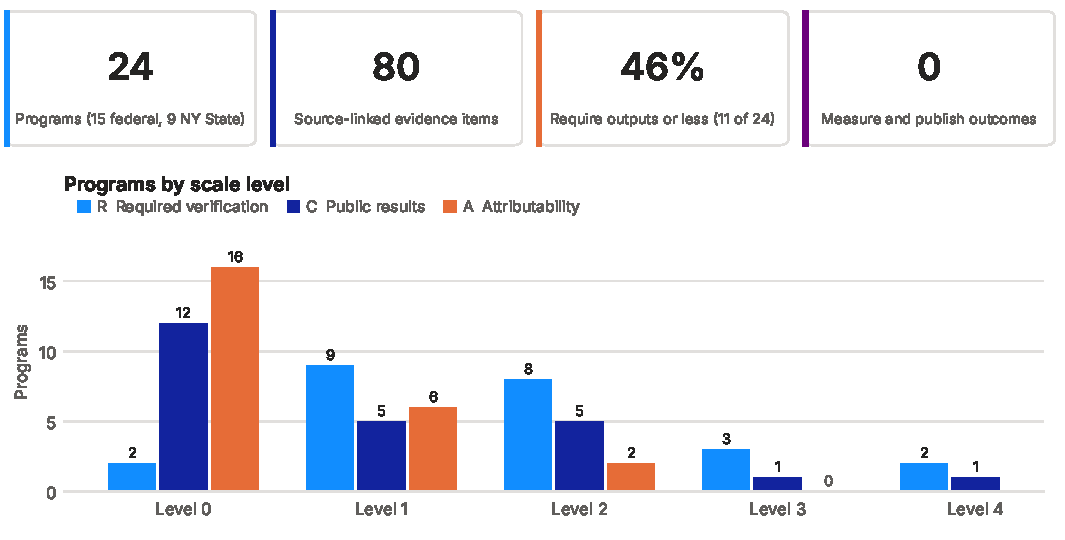
\includegraphics[width=\textwidth]{figures/fig1_overview.pdf}
\caption{Overview of Verification Gap Ledger v\vglVersion. Cards report the size of the register and two headline indicators; the clustered columns show the number of programs at each level of the three scales. The attributability scale has no level 4. No program both requires measured or independently verified outcomes and publishes project-level outcomes.}
\label{fig:overview}
\end{figure*}

\begin{table}[t]
\caption{Number of programs at each code level, and mean code, for the three scales ($n = \nProg$).}
\label{tab:dist}
\footnotesize
\setlength{\tabcolsep}{4pt}
\begin{tabular}{l ccccc c}
\toprule
Scale & 0 & 1 & 2 & 3 & 4 & Mean \\
\midrule
\tabinput{tab_dist.tex}
\bottomrule
\end{tabular}
\end{table}

Public results are lower than required verification. Of the \nProg{} programs, \nCzero{} (\pctCzero{} percent) publish no results beyond award announcements or recipient lists ($C = 0$). Of the remainder, \nCone{} publish aggregate results only, \nCtwo{} publish project-level outputs, \nCthree{} publishes project-level outcomes, and \nCfour{} publishes project-level outcome fields as bulk machine-readable open data. The mean $C$ code is \meanC, against a mean $R$ code of \meanR.

Attributability is the weakest dimension. A total of \nAzero{} programs (\pctAzero{} percent) have no required or published baseline ($A = 0$), \nAone{} have a baseline or modeled counterfactual only, and \nAtwo{} have measured pre and post outcomes at project level. No program is coded $A = 3$. In total, \nAleOne{} programs (\pctAleOne{} percent) are coded $A \le 1$, and the mean $A$ code is \meanA. Codes therefore fall from the rules programs set ($R$), to what they publish ($C$), to what could support attribution ($A$).

\subsection{Required verification against public results}

Figure~\ref{fig:matrix} places each program by its $R$ and $C$ codes, and Fig.~\ref{fig:gap} shows the gap $G_i$ of Eq.~(\ref{eq:gap}) for every program. A total of \nGapPos{} programs (\pctGapPos{} percent) have a positive gap, meaning their rules require more proof than they publish; \nGapNeg{} have a negative gap and \nGapZero{} a gap of zero. The mean outcome gap of Eq.~(\ref{eq:og}) is $\bar{O} = \meanOG$ on a scale where 0 is best.

\begin{figure}[t]
\centering
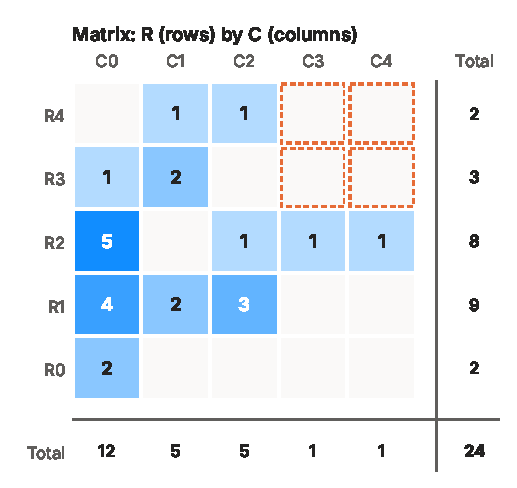
\includegraphics[width=\columnwidth]{figures/fig2_matrix.pdf}
\caption{Matrix of programs by required verification $R$ (rows) and public results $C$ (columns), with row and column totals. Cell shading scales with the number of programs. The dashed cells mark the region $R \ge 3$ and $C \ge 3$, which identifies programs that both measure and publish project-level outcomes; it is empty.}
\label{fig:matrix}
\end{figure}

The two quadrants that matter most are empty. No program that requires measured or independently verified outcomes ($R \ge 3$) publishes project-level outcomes ($C \ge 3$). Conversely, the two programs that do publish project-level outcomes, the Congestion Mitigation and Air Quality Improvement Program ($R = 2$, $C = 3$) and Building Resilient Infrastructure and Communities ($R = 2$, $C = 4$), publish modeled estimates: ex ante emissions reductions against a no-build case for CMAQ, and benefit cost ratios against a modeled no-action baseline for BRIC \cite{srcF006,srcF012}. In this sample, the programs that publish outcomes do not measure them, and the programs that measure outcomes do not publish them at project level.

The five programs coded $R \ge 3$ illustrate the pattern. NEVI and the Charging and Fueling Infrastructure grants require quarterly metered operating data per charging port under 23 CFR 680.112, but the regulation permits public release only in aggregated and anonymized form, and a national aggregate release had not been confirmed at the time of coding ($C = 1$) \cite{srcF007}. The Grid Resilience formula grants require reliability indices such as SAIDI and SAIFI measured before and after implementation, but no public release of subrecipient impact data was located ($C = 0$) \cite{srcF002}. NYSERDA's Clean Energy Communities and Real Time Energy Management programs have been subject to third-party impact evaluations whose results are public at program level only ($C = 2$ and $C = 1$) \cite{srcNY001,srcNY002}.

\begin{figure}[t]
\centering
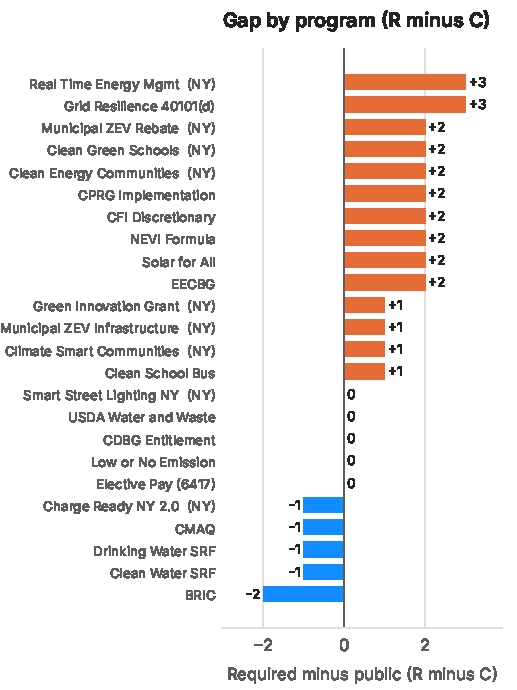
\includegraphics[width=\columnwidth]{figures/fig3_gap.pdf}
\caption{Required-to-public gap $G_i = R_i - C_i$ for every program, sorted. Positive bars (orange) mark programs whose rules require more verification than they publish; negative bars (blue) mark programs that publish more than their rules require, mostly through agency data portals. NY marks New York State programs.}
\label{fig:gap}
\end{figure}

Programs with a negative gap publish more than their rules require. They are concentrated among programs served by agency data systems: the EPA State Revolving Fund public portal \cite{srcF003}, the FHWA CMAQ Public Access System \cite{srcF006}, OpenFEMA \cite{srcF012}, and the New York open data portal for Charge Ready NY \cite{srcNY004}. Disclosure in these cases is a property of the agency's data infrastructure rather than of the reporting obligation placed on recipients.

\subsection{Association among the scales}

Table~\ref{tab:tau} and Fig.~\ref{fig:tau} report Kendall's $\tau_b$ of Eq.~(\ref{eq:tau}) for each pair of scales. Required verification and public results are weakly associated ($\tau_b = \tauRC$, $p = \pRC$). Required verification and attributability are strongly associated ($\tau_b = \tauRA$, $p < 0.001$), which is expected because a measured baseline is a precondition for both $R = 3$ and $A = 2$. Public results and attributability are weakly associated ($\tau_b = \tauCA$, $p = \pCA$). These coefficients indicate that the evidentiary strength of a program's rules is a poor guide to what it discloses.

\begin{table}[t]
\caption{Kendall's $\tau_b$ between pairs of scales, Eq.~(\ref{eq:tau}), with two-sided asymptotic $p$-values.}
\label{tab:tau}
\footnotesize
\begin{tabular}{l ccc}
\toprule
Pair & $\tau_b$ & $p$ & $n$ \\
\midrule
\tabinput{tab_tau.tex}
\bottomrule
\end{tabular}
\end{table}

\begin{figure}[t]
\centering
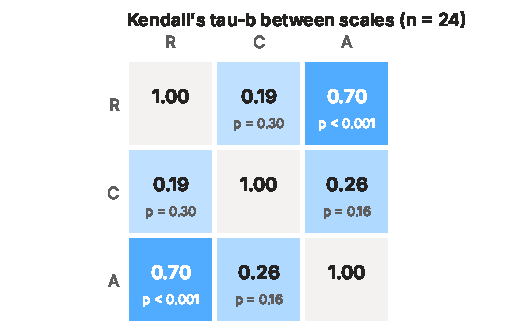
\includegraphics[width=0.92\columnwidth]{figures/fig7_tau.pdf}
\caption{Kendall's $\tau_b$ matrix for the three scales. Shading scales with the coefficient; each off-diagonal cell gives its two-sided $p$-value.}
\label{fig:tau}
\end{figure}

\subsection{Federal and state programs}

The federal and state subsamples show similar patterns (Table~\ref{tab:level}, Fig.~\ref{fig:level}). State programs have a higher mean required verification code, driven by the two NYSERDA programs with independent evaluations. Federal programs publish slightly more, driven by the OpenFEMA and CMAQ public data systems and the State Revolving Fund portal. Neither subsample contains a program that both measures and publishes project-level outcomes.

\begin{table}[t]
\caption{Summary indicators by level of government. Counts are numbers of programs; $G_i$ and $\bar{O}$ follow Eqs.~(\ref{eq:gap}) and (\ref{eq:og}).}
\label{tab:level}
\footnotesize
\setlength{\tabcolsep}{4pt}
\begin{tabular}{l ccc}
\toprule
Indicator & Federal & NY State & All \\
 & ($n = \nFed$) & ($n = \nNY$) & ($n = \nProg$) \\
\midrule
\tabinput{tab_level.tex}
\bottomrule
\end{tabular}
\end{table}

\begin{figure}[t]
\centering
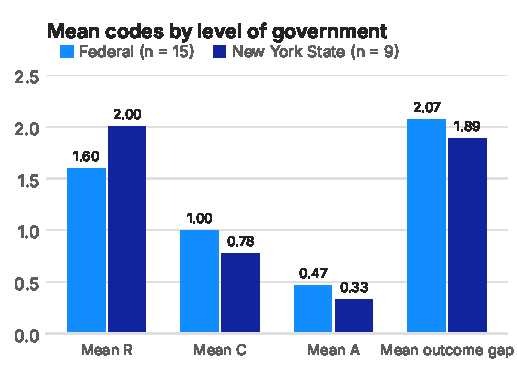
\includegraphics[width=\columnwidth]{figures/fig4_level.pdf}
\caption{Mean $R$, $C$, and $A$ codes and mean outcome gap $\bar{O}$ for federal and New York State programs.}
\label{fig:level}
\end{figure}

\subsection{Evidence confidence}

Confidence is uneven across dimensions (Table~\ref{tab:conf}, Fig.~\ref{fig:conf}). Required verification codes rest on low-confidence evidence for \nLowR{} programs. Low-confidence $R$ codes arise mainly where a program page defers reporting rules to award terms or application packages that were not reviewed. Public results codes are mostly medium confidence, because absence of publication is established by search of official channels rather than by a rule text. In total, \nLowR{} $R$ codes, \nLowC{} $C$ codes, and \nLowA{} $A$ codes rest on low-confidence evidence; Sec.~\ref{sec:sens} tests which findings depend on them.

\begin{table}[t]
\caption{Programs by confidence $\kappa_i^d$ of the evidence supporting each code, Eq.~(\ref{eq:conf}).}
\label{tab:conf}
\footnotesize
\begin{tabular}{l ccc}
\toprule
Dimension & High & Medium & Low \\
\midrule
\tabinput{tab_conf.tex}
\bottomrule
\end{tabular}
\end{table}

\begin{figure}[t]
\centering
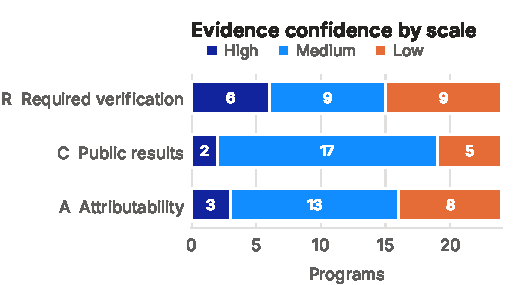
\includegraphics[width=\columnwidth]{figures/fig5_confidence.pdf}
\caption{Confidence of the evidence behind each program's code, by scale.}
\label{fig:conf}
\end{figure}

\subsection{What independent measurement shows}

The one program in the sample with a published billing-analysis evaluation shows why the distinction between estimated and measured outcomes matters. An independent impact evaluation of NYSERDA's Real Time Energy Management program applied IPMVP Option C whole-building billing analysis to 39 of 42 sampled sites and reported gross realization rates, Eq.~(\ref{eq:rr}), of $\rho = \rtemElec$ percent for electricity, \rtemFossil{} percent for fossil fuels, and \rtemComb{} percent combined; evaluated savings were about 3 percent of baseline use \cite{srcNY002}. Government facilities accounted for 17 of 293 projects and K-12 schools for 14. The evaluation measured pre and post consumption but did not use a comparison group or address net-to-gross attribution ($A = 2$). Figure~\ref{fig:rtem} shows the three rates against the estimate.

\begin{figure}[t]
\centering
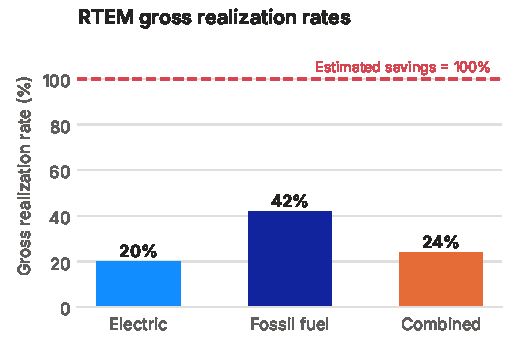
\includegraphics[width=\columnwidth]{figures/fig6_rtem.pdf}
\caption{Gross realization rates $\rho$ reported by the independent evaluation of NYSERDA's Real Time Energy Management program. The dashed line marks full realization of estimated savings ($\rho = 100$ percent).}
\label{fig:rtem}
\end{figure}

A single evaluation does not establish a general realization rate. It shows that reported estimates and measured results can diverge by a large margin, and that the divergence is visible only where measurement is required and its results are published.

% =====================================================================
\section{Interpretations}\label{sec:interp}

\subsection{Sensitivity to low-confidence codes}\label{sec:sens}

Because \nLowR{} $R$ codes, \nLowC{} $C$ codes, and \nLowA{} $A$ codes rest on low-confidence evidence, the headline indicators were recomputed under the four treatments of Eqs.~(\ref{eq:excl}) and (\ref{eq:shift}). Table~\ref{tab:sens} reports counts, and Fig.~\ref{fig:sens} shows the same indicators as shares of each sample so that the restricted samples can be compared with the full one.

\begin{table*}[t]
\caption{Headline indicators under alternative treatments of low-confidence codes, Eqs.~(\ref{eq:excl}) and (\ref{eq:shift}). Entries are numbers of programs.}
\label{tab:sens}
\footnotesize
\begin{tabular}{l ccccccc}
\toprule
Treatment & Programs & $R \le 1$ & $R \ge 3$ & $C = 0$ & $A \le 1$ & $R \ge 3$ and $C \ge 3$ & $G_i > 0$ \\
\midrule
\tabinput{tab_sens.tex}
\bottomrule
\end{tabular}
\end{table*}

\begin{figure*}[t]
\centering
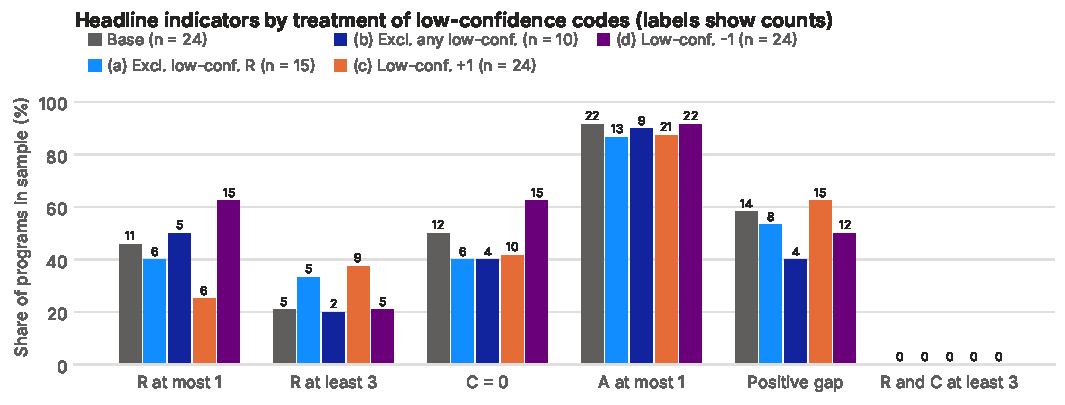
\includegraphics[width=\textwidth]{figures/fig8_sensitivity.pdf}
\caption{Headline indicators under the base codes and the four treatments of low-confidence codes, as shares of each sample; labels give counts. The joint indicator $R \ge 3$ and $C \ge 3$ is zero under every treatment.}
\label{fig:sens}
\end{figure*}

The central finding is stable. Under every treatment, no program both requires measured or verified outcomes and publishes project-level outcomes. At least \sensAleOneMin{} of \nProg{} programs in the full-sample treatments (and \sensBAleOne{} of \sensBProg{} in the most restricted sample) remain at or below a modeled baseline for attributability. The share of programs requiring outputs or less is the least stable indicator: across the full-sample treatments it ranges from \sensRleOneMin{} to \sensRleOneMax{} of \nProg{}, depending on how low-confidence $R$ codes are treated. Of the \nLowR{} low-confidence $R$ codes, \nLowRState{} belong to New York State programs whose reporting rules are set in requests for applications or award contracts not reviewed for version \vglVersion; those programs are the priority for review in version 0.5.

\subsection{Illustrative scenario: disclosure of collected outcome data}\label{sec:scenario}

To show how the Ledger can be used to evaluate a policy option, consider the scenario of Eq.~(\ref{eq:scen}), in which every program that already requires measured or independently verified outcomes publishes those outcomes at project level. The scenario changes no program's rules about what recipients must collect. It affects \scAffected{} programs: the Grid Resilience formula grants, NEVI, the Charging and Fueling Infrastructure grants, Clean Energy Communities, and Real Time Energy Management.

\begin{table}[t]
\caption{Indicators under current codes and under the disclosure scenario of Eq.~(\ref{eq:scen}).}
\label{tab:scen}
\footnotesize
\begin{tabular}{l cc}
\toprule
Indicator & Current & Scenario \\
\midrule
\tabinput{tab_scen.tex}
\bottomrule
\end{tabular}
\end{table}

Under the scenario (Table~\ref{tab:scen}, Fig.~\ref{fig:scen}), the number of programs that both measure and publish project-level outcomes rises from \nBoth{} to \scBothAfter, the number with a positive gap falls from \nGapPos{} to \scGapAfter, and the mean $C$ code rises from \meanC{} to \scMeanCAfter. Programs with no public results fall from \nCzero{} to \scCzeroAfter. The attributability distribution is unchanged, because publication does not create a baseline that was not collected. However, two of the five programs, Grid Resilience and Real Time Energy Management, would then publish measured pre and post data that outside analysts could pair with comparison sites, which is the step from $A = 2$ to $A = 3$ that no program in the sample has taken.

\begin{figure}[t]
\centering
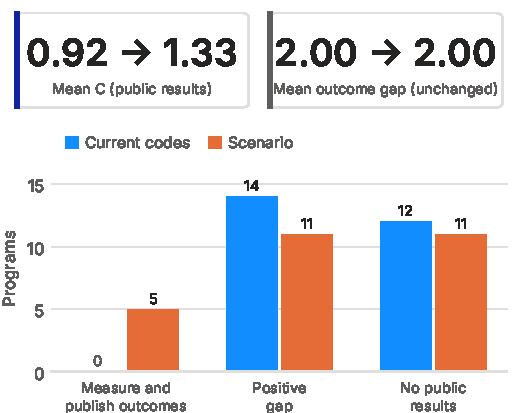
\includegraphics[width=\columnwidth]{figures/fig9_scenario.pdf}
\caption{Disclosure scenario of Eq.~(\ref{eq:scen}). Columns compare three indicators under current codes and under the scenario; cards show the change in mean $C$ and the unchanged mean outcome gap.}
\label{fig:scen}
\end{figure}

The scenario also exposes a property of the outcome gap derived in Sec.~\ref{sec:framework}: because $O_i = 4 - \max(R_i, C_i)$, it does not change when a program that already measures begins to publish, and the mean stays at \meanOG. The outcome gap therefore measures distance from the strongest evidence level on either scale, not alignment between them, and should be read together with the required-to-public gap. Version 1.0 will consider a joint indicator that rewards measured outcomes only when they are also published.

This scenario is illustrative. It is not a recommendation that any agency adopt a specific disclosure rule, and it does not account for confidentiality constraints, such as the anonymization clause in 23 CFR 680.112 or taxpayer confidentiality for elective pay, that may limit project-level release.

\subsection{Policy implications}

\textit{Collection and disclosure are separate decisions.} The strength of a program's verification requirements says little about what it discloses. Programs that require metered or independently verified outcomes keep those data internal or release them in aggregate, while the programs with the most open project-level data systems publish modeled estimates. For municipal officials, a program's published figures cannot be read as evidence of realized performance without checking how they were produced. For oversight bodies, a finding of weak disclosure does not imply weak collection, and the reverse.

\textit{The federal floor permits output-only reporting.} In the sample, \nRleOne{} programs require no more than output reporting, consistent with a Uniform Guidance that recommends rather than requires baselines and outcome indicators. Agencies that wish to support later evaluation can specify baseline and outcome data in award terms, as DOE did in the Grid Resilience metrics guidance \cite{srcF002} and FHWA did in 23 CFR 680.112 \cite{srcF007}. These cases show that measurement requirements can be written into program rules for municipal recipients without an evaluation contract.

\textit{Attribution requires design choices made before funding.} No program is coded $A = 3$, and only \nAtwo{} support measured pre and post comparison. Attribution cannot be added after the fact if baselines were not collected. Where programs already require metered operating data, publishing those data at project level with appropriate anonymization would allow independent analysts to construct comparison groups. Where programs fund equipment with predictable energy profiles, such as street lighting conversions or fleet replacement, a simple pre and post consumption requirement would move a program from $A = 0$ to $A = 2$.

\textit{Municipal decision support.} Municipalities choosing among funding sources typically compare eligibility, match requirements, and award size. The Ledger adds a further dimension: the evidence a program will generate. A municipality that wants to demonstrate realized savings to its governing body, bond investors, or residents may prefer programs that require measured outcomes, or may collect measured data voluntarily where rules do not require it. Because the Ledger is open and versioned, its codes can be incorporated into municipal planning and decision-support tools.

\textit{Evaluation and oversight.} The Ledger identifies where independent evidence exists and where it does not. Programs coded $R = 2$ with $C \ge 3$, which publish project-level estimates, are candidates for retrospective validation against utility or operating data. Programs coded $R \ge 3$ with $C \le 1$ are candidates for requests to release existing measured data. Programs coded $R \le 1$ cannot be validated from program records at all.

% =====================================================================
\section{Limitations}\label{sec:limits}

The findings should be read with the following limitations.
\begin{enumerate}
\item \textit{Publication, not collection.} $C$ measures what is public. Agencies may hold outcome data they do not release, and $C = 0$ means no public results were found through official channels, not that none exist.
\item \textit{Purposive sample.} The \nProg{} programs were chosen to span agencies, funding vehicles, and asset classes. They are not a random or complete sample, and the distributions describe these programs only.
\item \textit{Single coder.} Every code was assigned by one coder and confirmed by the maintainer against its cited source. Inter-coder agreement will first be reported in version 0.5.
\item \textit{Secondary official material.} Many program pages defer reporting rules to award terms or application packages that were not reviewed. These codes carry low confidence, and Sec.~\ref{sec:sens} shows which findings depend on them.
\item \textit{Changing requirements.} Several programs were suspended, rescinded, terminated, or litigated in 2025 and 2026. Codes reflect sources accessed in October 2026.
\item \textit{Ordinal scales.} The derived measures of Eqs.~(\ref{eq:gap}) and (\ref{eq:og}) subtract ordinal codes for convenience, and means of codes are summaries only.
\item \textit{Design, not performance.} The Ledger rates what programs require and publish. It does not judge whether any project saved energy or reduced emissions.
\item \textit{Tax credits at the mechanism level.} Elective pay is coded as a single mechanism, although production-based credits use metered output and investment-based credits are cost based.
\item \textit{Manual retrieval.} Sources were read through a web reader and logged by hand with URL and access date, not retrieved by scripted download with checksums, and some may move or change after the access date.
\item \textit{Documentation counts.} The version \vglVersion{} codebook lists 79 evidence rows and 4 reference sources, while the released tables contain \nEvid{} evidence rows and 3 reference sources. This paper uses the released tables; the codebook will be corrected in the next release.
\end{enumerate}

% =====================================================================
\section{Concluding remarks}\label{sec:concl}

Public programs funding municipal energy and infrastructure differ widely in the evidence they generate, and those differences have not previously been recorded in one public, source-cited register. In this work we introduced the Verification Gap Ledger, which separates three properties that are often conflated: what verification a program requires, what results it publishes, and whether its data could support attribution of outcomes to the funding.

In the first sample of \nProg{} federal and New York State programs, \pctRleOne{} percent require no more than output reporting, \pctCzero{} percent publish no results beyond award announcements, and \pctAleOne{} percent are coded at or below a modeled baseline for attributability. No program both requires measured or independently verified outcomes and publishes them at project level, and this finding holds under every sensitivity treatment tested. The programs that publish project-level outcomes publish modeled estimates, and the one program with a published billing-analysis evaluation measured electric savings at \rtemElec{} percent of estimates. Required verification and disclosure are only weakly associated ($\tau_b = \tauRC$). Together these results indicate that, for most programs in the sample, the realized effects of public spending on municipal energy and infrastructure cannot be confirmed from public records.

The Ledger is designed to grow and to be tested. Version 0.5 (February 2027) will review award terms for low-confidence codes and introduce an independent second coder on a random 20 percent sample, reporting percent agreement and weighted kappa. Version 1.0 (May 2027) will expand program coverage and refine the derived indicators, including a joint measured-and-published indicator motivated by Sec.~\ref{sec:scenario}. Version 2.0 (December 2027) will extend coverage further and maintain the register as a searchable public resource. Every code change is recorded with its reason, and identifiers remain permanent. Researchers, program staff, and municipal officials who identify a program that should be added or a code that should be reconsidered can submit the source through the public repository.

\section*{Data and code availability}

All data, documentation, and code are openly available. Version \vglVersion{} of the Verification Gap Ledger is archived on Zenodo at \href{https://doi.org/10.5281/zenodo.23302898}{doi:10.5281/zenodo.23302898}; the concept DOI \href{https://doi.org/10.5281/zenodo.23302897}{10.5281/zenodo.23302897} resolves to the latest version. The source repository is \url{https://github.com/Olumide-Akindipe/verification-gap-ledger}, and the Ledger can be browsed and searched at \url{https://olumide-akindipe.github.io/verification-gap-ledger}. Every number, table, and figure in this paper is produced from vgl\_programs.csv and vgl\_evidence.csv by the repository scripts 01\_build.py, 05\_preprint\_stats.py, and 06\_preprint\_assets.py, and recorded in stats.json and stats\_preprint.json. Data and documents are licensed CC BY 4.0; code is licensed MIT.

\section*{Declarations}

\textit{Funding.} This research received no external funding. \textit{Competing interests.} The author declares no competing interests. \textit{Author contributions (CRediT).} Stephen Olumide Akindipe: conceptualization, methodology, data curation, investigation, validation, software, writing (original draft, review and editing).

\bibliographystyle{unsrtnat}
\bibliography{refs_main,refs_programs}

% =====================================================================
\appendix
\renewcommand{\thetable}{A\arabic{table}}
\setcounter{table}{0}
\onecolumn
\section*{Appendix A: Codes for all programs}

\begin{table}[h]
\caption{Verification Gap Ledger v\vglVersion{} codes for all \nProg{} programs. $G$ and $O$ are the gap and outcome gap of Eqs.~(\ref{eq:gap}) and (\ref{eq:og}). Confidence is listed in $R$/$C$/$A$ order (H high, M medium, L low). Ev. is the number of evidence items. Program-level sources for every code are listed with URL, locator, and access date in vgl\_evidence.csv.}
\label{tab:appendix}
\footnotesize
\begin{tabular}{l L{8.6cm} ccccc c c}
\toprule
Ledger ID & Program & $R$ & $C$ & $A$ & $G$ & $O$ & Conf. & Ev. \\
\midrule
\tabinput{tab_appendix.tex}
\bottomrule
\end{tabular}
\end{table}

\end{document}
